\section{Protocolo NTP}
\label{sec:NTP}

O Network Time Protocol é um protocolo de sincronização
de relógios que sincroniza os relógios de um sistema distribuído 
através de redes com comutação de pacotes e de latência variável 
com uma precisão na ordem dos milissegundos. Este protocolo
foi primordialmente concebido para ter uma alta exatidão 
e fiabilidade \cite{b2}.

Para uma típica operação do protocolo NTP,
o cliente questiona um ou mais servidores NTP, de modo a 
receber o tempo atualizado. Após a receção dos dados do servidor, 
o cliente calcula o offset do seu relógio relativamente ao servidor, o delay da rede e o rate. Para tal, é necessário q ele saiba os timestamps da mensagem enviada por ele ao servidor e da consequente resposta do servidor,
para tal figura \ref{fig:diagramaNTP} contextualiza o protocolo de melhor
forma. Os timestamps que são necessário são então o tempo a que
a mensagem foi enviada pelo cliente, t0, e quando foi recebida pelo
servidor, t1, tal como quando a mensagem de resposta foi enviada
pelo servidor, t2, e finalmente recebida pelo cliente, t3.

    \begin{figure}[h]
        \centering
        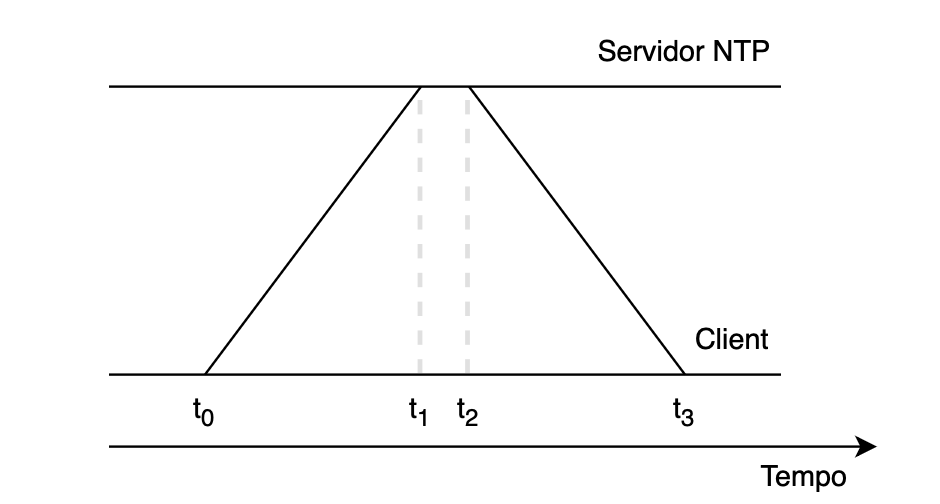
\includegraphics[width=0.8\linewidth]{figures/diagramaNTP.png}
        \caption{Ordem de eventos do protocolo NTP}
        \label{fig:diagramaNTP}
    \end{figure}

Com estes 4 tempos é então possível calcular quer o valor do offset quer o valor 
do delay da rede. O offset, $\theta$, vai corresponder 
à diferença entre o relógio do cliente e do servidor, sendo o valor dado pela equação \ref{eq:offset}. 


\begin{equation} \label{eq:offset}
\theta = \frac{\left( (t_{\text{1}} - t_{\text{0}}) + (t_{\text{2}} - t_{\text{3}}) \right)}{2} 
\end{equation}

O delay da rede, $\delta$, corresponde por sua vez ao tempo
que um pacote demora a ir do cliente ao servidor e vice-versa, sendo
o valor dado pela equação \ref{eq:delay}.


\begin{equation} \label{eq:delay}
\delta = (t_{\text{3}} - t_{\text{0}}) - (t_{\text{2}} - t_{\text{1}})
\end{equation}

Para além disso também pode ser calculado o rate, que serve
para compensar o desvio do relógio do cliente quando comparado com o do servidor.
Para tal, para o sistema criado no âmbito do projeto definiu-se a função do
rate de acordo com a equação \ref{eq:rate}. Na equação apresentada,
o valor $t_{\text{3}}'$ e $t_{\text{1}}'$ correspondem aos timestamps 
mais recentes, enquanto t1 e t3 correspondem aos timestamps da mensagem anterior à
atual. Assim, o rate vai sendo modificado com base nos timestamps
das duas últimas iterações entre cliente-servidor.


\begin{equation} \label{eq:rate}
\text{{rate}} =\left| \frac{{t_{\text{1}}' - t_{\text{1}} - \delta + \delta '}}{{t_{\text{3}}' - t_{\text{3}}}} \right|
\end{equation}


Por fim, a equação \ref{eq:corrected_time} foi concebida, de modo a corrigir
o tempo do relógio do cliente, sendo a variável \text{{elapsed\_time}} o tempo
que entre $t_{\text{3}}$ e o tempo em que a correção do tempo foi efetuada.


\begin{equation} \label{eq:corrected_time}
\text{{corrected\_time}} = t_{\text{3}} + \text{{elapsed\_time}} \cdot \text{{rate}} + \theta
\end{equation}


